\documentclass{standalone}
\usepackage{tikz}

\begin{document}
	
	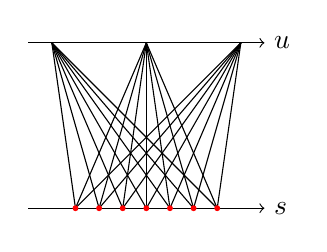
\begin{tikzpicture}[scale = 0.3]
		
		\draw[->] (-2, 0) -- (8, 0);
		\draw[->] (-2, 7) -- (8, 7);
		
		\node[right] at (8, 0) {$s$};
		\node[right] at (8, 7) {$u$};
		
		\draw (-1, 7) -- (0, 0);
		\draw (-1, 7) -- (1, 0);
		\draw (-1, 7) -- (2, 0);
		\draw (-1, 7) -- (3, 0);
		\draw (-1, 7) -- (4, 0);
		\draw (-1, 7) -- (5, 0);
		\draw (-1, 7) -- (6, 0);
		
		\draw (3, 7) -- (0, 0);
		\draw (3, 7) -- (1, 0);
		\draw (3, 7) -- (2, 0);
		\draw (3, 7) -- (3, 0);
		\draw (3, 7) -- (4, 0);
		\draw (3, 7) -- (5, 0);
		\draw (3, 7) -- (6, 0);
		
		\draw (7, 7) -- (0, 0);
		\draw (7, 7) -- (1, 0);
		\draw (7, 7) -- (2, 0);
		\draw (7, 7) -- (3, 0);
		\draw (7, 7) -- (4, 0);
		\draw (7, 7) -- (5, 0);
		\draw (7, 7) -- (6, 0);
		
		\draw[fill, red] (0, 0) circle [radius = 0.1];
		\draw[fill, red] (1, 0) circle [radius = 0.1];
		\draw[fill, red] (2, 0) circle [radius = 0.1];
		\draw[fill, red] (3, 0) circle [radius = 0.1];
		\draw[fill, red] (4, 0) circle [radius = 0.1];
		\draw[fill, red] (5, 0) circle [radius = 0.1];
		\draw[fill, red] (6, 0) circle [radius = 0.1];
		
	\end{tikzpicture}
	
\end{document}